\documentclass[a4paper,11pt]{article}
\usepackage[italian]{babel}
\usepackage[utf8]{inputenc}
\usepackage{graphicx}
\usepackage{epstopdf}
\usepackage[labelfont=bf]{caption}

\author{A.~Battistello\and P.~Ferretti}
\title{Machine Learning techniques to Model Data Intensive Application Performance}
\date{\today}
\begin{document}
\maketitle
\tableofcontents
\section{Prime analisi}
\subsection{SVR vs Linear Regression}
Presa in considerazione la query R2, cerchiamo di prevedere il tempo di esecuzione della query con 80 cores. \newline
Creeremo i nostri modelli facendo training su numeri di cores diversi da quello di test: 60, 72, 90, 100, 120. \newline
Dai risultati potremo confrontare la performance della regressione lineare rispetto a vari modelli di Support Vector Regression (lineare, polinomiale, sigmoidale). \newline
\newline
Come si può vedere dalla Tabella \ref{tabletest1} i risultati migliori si hanno dalla SVR lineare, mentre gli altri due tipi di SVR sono addirittura peggiori della semplice regressione lineare, probabilmente per problemi di \textit{overfit}.
\newline

\begin{table}[bht]
\centering
\label{tabletest1}
\begin{tabular}{c | c c p{2cm} p{2cm} p{2cm}}
Modello & RMSE & R\textsuperscript{2} & Errore assoluto medio & Errore relativo medio & Differenza medie \tabularnewline
\hline
Regressione lineare & 0.0940 & 0.9952 & 213397 & 0.0295 & -0.0378 \\
SVR lineare & 0.0722 & 0.9991 & 220018 & 0.1730 & 0.0526\\
SVR polinomiale & 0.1050 & 0.9976 & 226093 & 0.1831 &0.0780\\
SVR sigmoidale & 0.5862 & 0.9802 & 279777 & 0.2286 & -0.2487
\end{tabular}
\\
\caption{Risultati per il primo test}
\end{table}

\begin {figure}
\centering
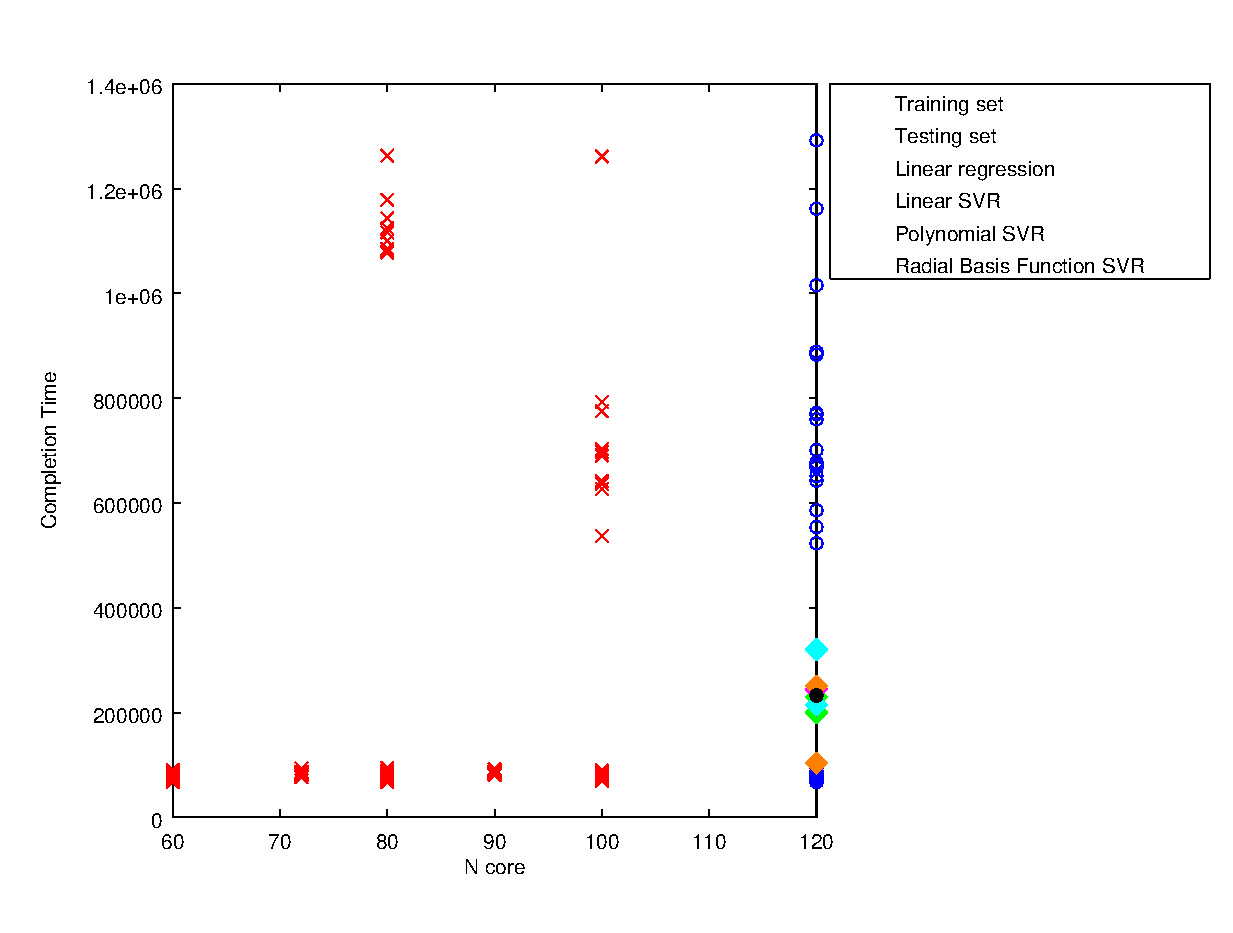
\includegraphics[width=\textwidth]{outputPlots/plot_Ncore.eps}
\caption {Test su numero di cores. La croce nera indica la media originale dei valori di test.}
\end {figure}

\end{document}
